\documentclass[]{politex}

% ========== Packages ==========
\usepackage[utf8]{inputenc}
\usepackage{amsmath,amsthm,amsfonts,amssymb}
\usepackage{graphicx,cite,enumerate}
\graphicspath{ {images/}{../images/} }
\usepackage{tabularx}
\usepackage{longtable}
\usepackage{subfiles}
\usepackage{subcaption}
\usepackage{multirow}
\usepackage{float}
\usepackage[table,xcdraw]{xcolor}
\usepackage{listings}
\usepackage{pdfpages}
\usepackage{booktabs}
\usepackage[utf8]{inputenc}
\usepackage{makecell}
\usepackage[hidelinks]{hyperref}

\renewcommand\theadalign{bc}
\renewcommand\theadfont{\bfseries}
\renewcommand\theadgape{\Gape[4pt]}
\renewcommand\cellgape{\Gape[4pt]}

% ========== Language options ==========
\usepackage[brazil]{babel}
%\usepackage[english]{babel}


% ========== ABNT (requer ABNTeX 2) ==========
%	http://www.ctan.org/tex-archive/macros/latex/contrib/abntex2
\usepackage[num]{abntex2cite}

% Forçar o abntex2 a usar [ ] nas referências ao invés de ( )
\citebrackets{[}{]}


% ========== Lorem ipsum ==========
\usepackage{blindtext}

% ========== Fonte Sans Serif ==========
\renewcommand{\familydefault}{\sfdefault}

% ========== Opções do documento ==========
% Título
\titulo{Rede de Dispositivos para Monitoramento de qualidade e conforto em escritórios}

% Autor
\autor{Isabella Bologna Salomão\\%
		Renato de Oliveira Freitas}


% Orientador / Coorientador
\orientador{Prof. Dr. Gustavo P. Rehder\\%
			Prof.ª Dra. Cíntia Borges Margi}
% \coorientador{PullUp \\%
%             Eng. Conrado Leite de Vitor }

% Tipo de documento
% \tcc{Eletricista com ênfase em Eletrônica e Sistemas}
\tcc{Eletricista com ênfase em Computação}
% \dissertacao{Engenharia Elétrica}
%\teseDOC{Engenharia Elétrica}
%\teseLD
%\memorialLD

% Departamento e área de concentração
\departamento{PSI - Eletrônica e Sistemas}
\departamento{PCS - Computação e Sistemas Digitais}
\areaConcentracao{Engenharia Elétrica}


% Local
\local{São Paulo}

% Ano
\data{2020}


\begin{document}
% ========== Capa e folhas de rosto ==========
\capa

\falsafolhaderosto

\folhaderosto
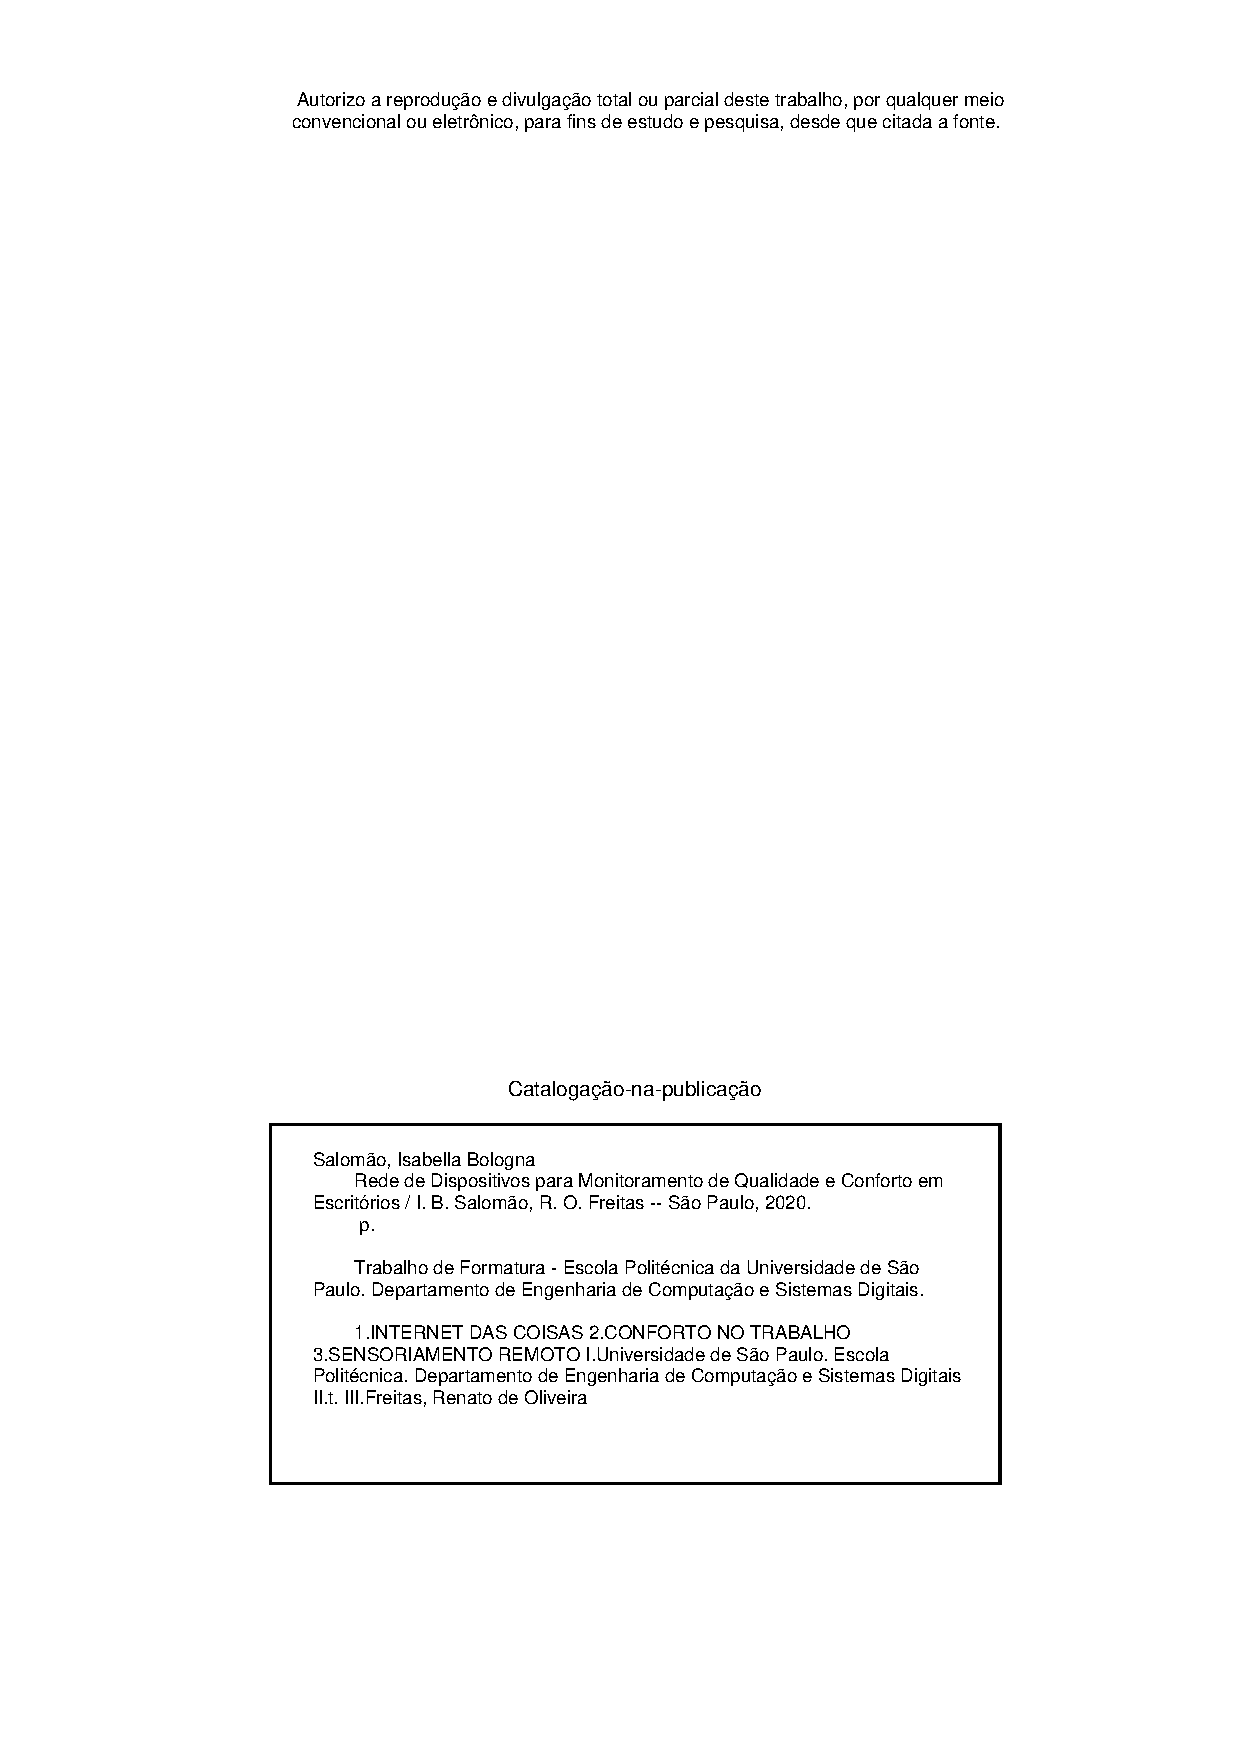
\includepdf{EPUSP-Catalogacao-na-Fonte.pdf}

\assinatura{Prof.ª Dra. Cíntia Borges Margi}
\assinatura{Prof. Dr. Gustavo P. Rehder}

\dedicatoria{Dedicamos esse trabalho aos amigos da equipe ThundeRatz}

\begin{agradecimentos}
	Ao nosso amigo Thalles Carneiro, que nos ajudou diretamente no desenvolvimento do projeto. 
	
	Aos nossos orientadores, Gustavo Rehder e Cintia Margi, por toda a ajuda e no quanto nos ensinaram ao longo do ano. Ao técnico Carlos Ramos do LME que nos ajudou nos testes do projeto, e ao professor Vitor Nascimento do PSI que nos tirou muitas dúvidas no desenvolvimento do projeto. 

	\hfill \break
	
	Isabella: Á minha família, minha mãe Rosangela, meu irmão Leonardo, meu pai Moacir e meu companheiro Kim, que me apoiaram para chegar até aqui. 
 
	Aos amigos que fiz na ThundeRatz, em especial ao Gustavo Hama, Renzo Abensur, Lucas Haug, Leonardo Baltazar, Felipe Gomes, Jean Mello e Gustavo Barranova pelo companheirismo ao longo desse ano tão peculiar e terem me ajudado na jornada do autoconhecimento. Ao restante da equipe pelos anos incríveis e os ensinamentos que levarei para a vida toda. 
	
	Aos meus amigos do Jaraguá, Guilherme, Flavio, Lucas Bredariol, Catarine, Lucas Botassio e Igor, colegas desde a infância e que se mantem presentes mesmo com a distância física.

	\hfill \break

	Renato: 
\end{agradecimentos}

\epigrafe{%
	\emph{``Amigo é um mago do meigo abraço"}
	\begin{flushright}
		(Emicida)
	\end{flushright}
}

% ========== Resumo ==========
\begin{resumo}

Soluções para o monitoramento de parâmetros que remetem à qualidade e conforto de ambientes internos vêm se tornando interessantes, dado ao aumento no tempo que pessoas passam nesse tipo de ambiente, como escritórios. A partir da coleta desses dados, é possível adotar medidas para tornar o local estudado mais saudável e confortável para as pessoas ali presentes. O objetivo deste trabalho é desenvolver uma rede de dispositivos eletrônicos \textit{Open Source} capaz de monitorar escritórios fechados, realizando a medição através de sensores de dados referentes à qualidade do ar, temperatura, luminosidade e ruído, além de coletar a opinião das pessoas sobre sua sensação de conforto no ambiente, para apresentar relatórios sobre o local em uma plataforma, que pode ser utilizada como base para tomar ações a fim de garantir o conforto de seus ocupantes. A rede de dispositivos proposta é implementada utilizando o protocolo \textit{Bluetooth Mesh}, uma tecnologia que aparece cada vez mais no escopo de Internet das Coisas e ambientes inteligentes, em conjunto com Wi-Fi e o protocolo MQTT, visando enviar os dados coletados pelos diversos sensores para uma plataforma hospedada em nuvem. 
%
\\[3\baselineskip]
%
\textbf{Palavras-Chave} -- Rede de Sensores Sem Fio. Internet das Coisas. Rede Bluetooth Mesh. Escritório Inteligente. 
\end{resumo}

\begin{abstract}
Solutions for monitoring parameters that refer to quality and comfort of indoor environments have become interesting, given the increasing time that people spend in this type of places, such as offices. Based on the collection of this data, it is possible to take action to make the studied place healthier and more comfortable for the people in it. The main goal of this work is to develop an  Open Source electronic device network capable of watching out closed office environments, using sensors to take measurements of air quality, temperature, luminosity and noise and, in addition, acquire people`s opinions on their sensation of comfort at the given place, to present data reports in a selected platform that can be used to take actions in order to ensure comfort and the overall environment quality. The proposed device network is implemented by using the Bluetooth Mesh protocol, a growing technology used more and more on the Internet of Things and smart enviroment applications, in addition to Wi-Fi and MQTT protocols, aiming to send the collected data to a cloud platform.
%
\\[3\baselineskip]
%
\textbf{Keywords} -- Wireless Sensor Network. Internet of Things. Bluetooth Mesh Network. Smart Office.
\end{abstract}

% ========== Listas (opcional) ==========
\listadefiguras
\listadetabelas


% ========== Sumário ==========
\sumario

% ========== Elementos textuais ==========

\chapter{Introdução} \label{cap:introducao}
\subfile{chapters/introducao}

\chapter{Estado da Arte e Trabalhos Relacionados} \label{cap:arte} % Tema? ~Estado da Arte~ 
\subfile{chapters/arte}

\chapter{Especificação}
\subfile{chapters/specs}

\chapter{Desenvolvimento}
\subfile{chapters/dev}

\chapter{Verificação do Projeto}
\subfile{chapters/resultados}

\chapter{Considerações Finais}
\subfile{chapters/conclusao}

\appendix
\chapter{Imagens}
\subfile{chapters/anexo}


% ========== Referências ==========
% --- IEEE ---
%	http://www.ctan.org/tex-archive/macros/latex/contrib/IEEEtran
%\bibliographystyle{IEEEbib}

% --- ABNT (requer ABNTeX 2) ---
%	http://www.ctan.org/tex-archive/macros/latex/contrib/abntex2
\bibliographystyle{abntex2-num}

\bibliography{reference}

\end{document}